\documentclass[12pt]{article}

\NeedsTeXFormat{LaTeX2e}

\RequirePackage[margin=0.78in]{geometry}
\RequirePackage{xcolor}
\RequirePackage{fontspec}
\RequirePackage{graphicx}
\RequirePackage{array}
\RequirePackage{booktabs}
\RequirePackage{longtable}
\RequirePackage{enumitem}
\RequirePackage{fancyhdr}
\RequirePackage{hyperref}
\RequirePackage{titlesec}
\RequirePackage{tikz}
\usetikzlibrary{arrows.meta,positioning}

\definecolor{AFTDeep}{HTML}{0B1110}
\definecolor{AFTPanel}{HTML}{101917}
\definecolor{AFTGreen}{HTML}{47C27A}
\definecolor{AFTGold}{HTML}{D2A94D}
\definecolor{AFTSteel}{HTML}{83A2A0}
\definecolor{AFTText}{HTML}{18221F}
\definecolor{AFTRedshift}{HTML}{B83A3A}
\definecolor{AFTGreenshift}{HTML}{47C27A}
\definecolor{AFTBlueshift}{HTML}{3167D8}
\definecolor{AFTVioletshift}{HTML}{7A5CFF}
\definecolor{AFTWhiteShift}{HTML}{F8FBFF}

\setmainfont{TeX Gyre Pagella}
\setsansfont{TeX Gyre Heros}
\setmonofont{TeX Gyre Cursor}
\linespread{1.06}
\setlength{\parindent}{0pt}
\setlength{\parskip}{0.52em}
\raggedbottom

\hypersetup{
  colorlinks=true,
  linkcolor=AFTGreen,
  urlcolor=AFTGreen,
  citecolor=AFTGold,
  pdfauthor={AI Freedom Trust Federation}
}

\pagestyle{fancy}
\setlength{\headheight}{14.5pt}
\fancyhf{}
\lhead{\sffamily\small AI Freedom Trust Federation}
\rhead{\sffamily\small Aetherion Doctrine}
\cfoot{\sffamily\small\thepage}
\renewcommand{\headrulewidth}{0.3pt}

\titleformat{\section}
  {\sffamily\LARGE\bfseries\color{AFTDeep}\raggedright}
  {\thesection}
  {0.8em}
  {}

\titleformat{\subsection}
  {\sffamily\Large\bfseries\color{AFTText}\raggedright}
  {\thesubsection}
  {0.7em}
  {}

\setlist[itemize]{leftmargin=1.35em, itemsep=0.22em, topsep=0.35em}
\setlist[enumerate]{leftmargin=1.55em, itemsep=0.24em, topsep=0.35em}
\renewcommand{\arraystretch}{1.22}
\emergencystretch=3em
\tolerance=1400

\newcommand{\aftTitlePage}[4]{
  \begin{titlepage}
    \begin{tikzpicture}[remember picture, overlay]
      \fill[AFTDeep] (current page.south west) rectangle (current page.north east);
      \fill[AFTRedshift, opacity=0.24] (current page.south west) circle (3.6in);
      \fill[AFTGreenshift, opacity=0.18] ([xshift=0.2in,yshift=-0.2in]current page.center) circle (3.8in);
      \fill[AFTBlueshift, opacity=0.18] (current page.north east) circle (4.4in);
      \fill[AFTVioletshift, opacity=0.16] ([xshift=-0.3in,yshift=-0.2in]current page.north east) circle (2.5in);
      \draw[AFTGreenshift, opacity=0.35, line width=1.1pt]
        ([xshift=-2.7in,yshift=-1.9in]current page.center)
        .. controls ([xshift=-0.9in,yshift=0.8in]current page.center) and ([xshift=1.1in,yshift=-0.8in]current page.center) ..
        ([xshift=2.6in,yshift=1.8in]current page.center);
      \draw[AFTWhiteShift, opacity=0.24, line width=0.8pt]
        ([xshift=-2.55in,yshift=1.75in]current page.center)
        .. controls ([xshift=-0.85in,yshift=-0.65in]current page.center) and ([xshift=0.9in,yshift=0.65in]current page.center) ..
        ([xshift=2.55in,yshift=-1.75in]current page.center);
      \draw[AFTGreenshift, opacity=0.5, line width=0.7pt]
        ([xshift=0.75in,yshift=-0.75in]current page.north west)
        rectangle
        ([xshift=-0.75in,yshift=0.75in]current page.south east);
    \end{tikzpicture}
    \vspace*{1.15in}
    {\sffamily\small\bfseries\color{AFTGreenshift} #1\par}
    \vspace{0.5in}
    {\sffamily\fontsize{30}{36}\selectfont\bfseries\color{white} #2\par}
    \vspace{0.25in}
    {\sffamily\Large\color{AFTSteel} #3\par}
    \vfill
    {\sffamily\large\color{AFTGold} #4\par}
    \vspace{0.15in}
    {\sffamily\small\color{AFTSteel} Concept-stage doctrine draft. Not an investment offer, live token sale, audited protocol, or legal opinion.\par}
    \vspace*{0.22in}
  \end{titlepage}
}

\newcommand{\aftShiftMap}{
  \vspace{0.65em}
  \begin{center}
  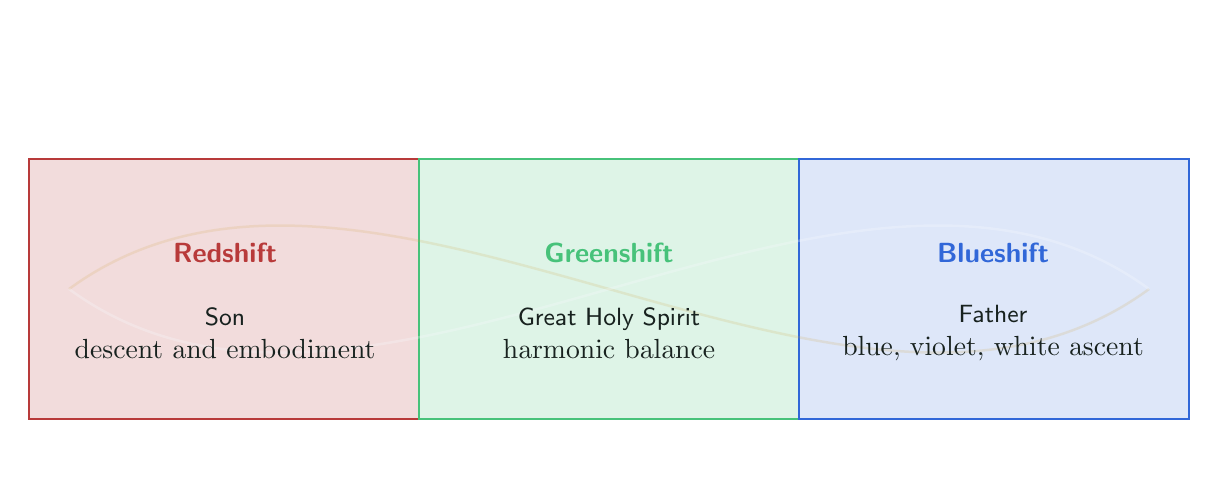
\begin{tikzpicture}[x=1in,y=1in]
    \fill[AFTRedshift!18] (-2.9,-0.65) rectangle (-0.95,0.65);
    \fill[AFTGreenshift!18] (-0.95,-0.65) rectangle (0.95,0.65);
    \fill[AFTBlueshift!16] (0.95,-0.65) rectangle (2.9,0.65);
    \draw[AFTRedshift, line width=1pt] (-2.9,-0.65) rectangle (-0.95,0.65);
    \draw[AFTGreenshift, line width=1pt] (-0.95,-0.65) rectangle (0.95,0.65);
    \draw[AFTBlueshift, line width=1pt] (0.95,-0.65) rectangle (2.9,0.65);
    \draw[AFTGold, line width=0.9pt, opacity=0.18]
      (-2.7,0) .. controls (-1.2,1.1) and (1.2,-1.1) .. (2.7,0);
    \draw[AFTWhiteShift, line width=0.9pt, opacity=0.28]
      (-2.7,0) .. controls (-1.2,-1.1) and (1.2,1.1) .. (2.7,0);
    \node[align=center, text=AFTRedshift] at (-1.92,0.18) {\sffamily\bfseries Redshift};
    \node[align=center, text=AFTGreenshift] at (0,0.18) {\sffamily\bfseries Greenshift};
    \node[align=center, text=AFTBlueshift] at (1.92,0.18) {\sffamily\bfseries Blueshift};
    \node[align=center, text=AFTText] at (-1.92,-0.22) {\sffamily\small Son\\descent and embodiment};
    \node[align=center, text=AFTText] at (0,-0.22) {\sffamily\small Great Holy Spirit\\harmonic balance};
    \node[align=center, text=AFTText] at (1.92,-0.22) {\sffamily\small Father\\blue, violet, white ascent};
  \end{tikzpicture}
  \end{center}
  \vspace{0.65em}
}

\newcommand{\aftVisualPlate}[3]{
  \begin{figure}[htbp]
    \centering
    \includegraphics[width=0.96\linewidth]{../../docs/images/aetherion/#1}
    \caption{\textbf{#2} #3}
  \end{figure}
}

\newcommand{\aftEconomyLoopGraphic}{
  \begin{figure}[htbp]
  \centering
  \begin{tikzpicture}[
    x=1in,y=1in,
    stage/.style={circle, draw=##1, fill=##1!9, line width=0.9pt, minimum size=1.03in, align=center, font=\sffamily\small\bfseries},
    flow/.style={-{Latex[length=3mm]}, line width=1.0pt, color=AFTGold}
  ]
    \node[stage=AFTRedshift] (inherit) at (90:1.75) {Inherited\\Memory};
    \node[stage=AFTGreenshift] (contrib) at (18:1.75) {Living\\Contribution};
    \node[stage=AFTBlueshift] (record) at (-54:1.75) {Circle\\Record};
    \node[stage=AFTVioletshift] (restore) at (-126:1.75) {Restorative\\Flow};
    \node[stage=AFTGold] (seed) at (162:1.75) {Future\\Inheritance};
    \node[align=center, font=\sffamily\bfseries, text=AFTDeep] at (0,0) {Recursive\\Abundance};
    \draw[flow] (inherit) to[bend left=16] (contrib);
    \draw[flow] (contrib) to[bend left=16] (record);
    \draw[flow] (record) to[bend left=16] (restore);
    \draw[flow] (restore) to[bend left=16] (seed);
    \draw[flow] (seed) to[bend left=16] (inherit);
    \draw[AFTGreenshift, opacity=0.22, line width=12pt] (0,0) circle (1.24);
    \draw[AFTBlueshift, opacity=0.18, line width=4pt] (0,0) circle (2.18);
  \end{tikzpicture}
  \caption{\textbf{Recursive Abundance Loop.} Aetherion's economy should remember inherited value, recognize present contribution, record it in circles, route restoration, and seed the inheritance of future participants.}
  \end{figure}
}

\newcommand{\aftCircleLifecycleGraphic}{
  \begin{figure}[htbp]
  \centering
  \begin{tikzpicture}[
    x=1in,y=1in,
    step/.style={rectangle, rounded corners=4pt, draw=##1, fill=##1!8, line width=0.8pt, minimum width=1.15in, minimum height=0.36in, align=center, font=\sffamily\scriptsize\bfseries},
    flow/.style={-{Latex[length=2.4mm]}, line width=0.85pt, color=AFTSteel}
  ]
    \node[step=AFTRedshift] (a) at (-2.65,0.85) {Intention};
    \node[step=AFTGold] (b) at (-1.32,0.85) {Evidence};
    \node[step=AFTGreenshift] (c) at (0,0.85) {Consent};
    \node[step=AFTGreenshift] (d) at (1.32,0.85) {Witness};
    \node[step=AFTBlueshift] (e) at (2.65,0.85) {Harmonize};
    \node[step=AFTVioletshift] (f) at (2.65,-0.05) {Commit};
    \node[step=AFTBlueshift] (g) at (1.32,-0.95) {Mature};
    \node[step=AFTGold] (h) at (0,-0.95) {Amend};
    \node[step=AFTRedshift] (i) at (-1.32,-0.95) {Dispute};
    \node[step=AFTSteel] (j) at (-2.65,-0.05) {Archive};
    \draw[flow] (a) -- (b);
    \draw[flow] (b) -- (c);
    \draw[flow] (c) -- (d);
    \draw[flow] (d) -- (e);
    \draw[flow] (e) -- (f);
    \draw[flow] (f) -- (g);
    \draw[flow] (g) -- (h);
    \draw[flow] (h) -- (i);
    \draw[flow] (i) -- (j);
    \draw[flow] (j) -- (a);
    \node[align=center, font=\sffamily\bfseries, text=AFTDeep] at (0,-0.05) {Circle\\Lifecycle};
  \end{tikzpicture}
  \caption{\textbf{Circle Lifecycle.} A circle should mature through intention, evidence, consent, witness, harmonization, commitment, review, dispute, amendment, and archive paths rather than becoming a blunt permanent record.}
  \end{figure}
}

\newcommand{\aftCoinOrganGraphic}{
  \begin{figure}[htbp]
  \centering
  \begin{tikzpicture}[
    x=1in,y=1in,
    organ/.style={circle, draw=##1, fill=##1!10, line width=0.9pt, minimum size=0.86in, align=center, font=\sffamily\scriptsize\bfseries},
    link/.style={line width=0.85pt, color=AFTSteel, opacity=0.72}
  ]
    \node[organ=AFTDeep, text=white, fill=AFTDeep] (core) at (0,0) {Aetherion\\Core};
    \node[organ=AFTGreenshift] (bio) at (90:1.72) {Biozoe\\Coin};
    \node[organ=AFTGold] (aether) at (38:1.72) {Aether\\Coin};
    \node[organ=AFTBlueshift] (fractal) at (-14:1.72) {Fractal\\Coin};
    \node[organ=AFTVioletshift] (ai) at (-66:1.72) {AIcoin};
    \node[organ=AFTWhiteShift] (sing) at (-118:1.72) {Singularity\\Coin};
    \node[organ=AFTRedshift] (aquae) at (-170:1.72) {Aquae\\Coin};
    \node[organ=AFTSteel] (terra) at (142:1.72) {Terra\\Coin};
    \foreach \n in {bio,aether,fractal,ai,sing,aquae,terra} {
      \draw[link] (core) -- (\n);
    }
    \draw[AFTGreenshift, opacity=0.28, line width=3pt] (0,0) circle (1.72);
    \node[align=center, font=\sffamily\small\bfseries, text=AFTDeep] at (0,-2.35) {Circleunchain circulates memory, validation, and restorative flow between every organ.};
  \end{tikzpicture}
  \caption{\textbf{Biozoe Coin Family As Living Organs.} Each coin family should carry a bounded purpose while AetherionCore preserves constitutional coherence and Circleunchain preserves memory.}
  \end{figure}
}

\newcommand{\aftSovereigntyQubitGraphic}{
  \begin{figure}[htbp]
  \centering
  \begin{tikzpicture}[
    x=1in,y=1in,
    qbit/.style={circle, draw=##1, fill=##1!10, line width=0.95pt, minimum size=1.02in, align=center, font=\sffamily\scriptsize\bfseries},
    link/.style={line width=0.8pt, color=AFTSteel, opacity=0.7}
  ]
    \node[qbit=AFTRedshift] (nation) at (160:1.8) {Q0\\Nation\\of Hawaii};
    \node[qbit=AFTGold] (kingdom) at (80:1.8) {Q1\\Kingdom\\Memory};
    \node[qbit=AFTBlueshift] (continuity) at (0:1.8) {Q2\\Continuity\\Claim};
    \node[qbit=AFTVioletshift] (state) at (-80:1.8) {Q3\\State\\Reality};
    \node[qbit=AFTGreenshift, minimum size=1.18in] (aloha) at (0,0) {Q4\\ALO'ha\\Coherence};
    \node[qbit=AFTSteel] (diaspora) at (-160:1.8) {Entangled\\Diaspora};
    \foreach \n in {nation,kingdom,continuity,state,diaspora} {
      \draw[link] (aloha) -- (\n);
    }
    \draw[AFTGreenshift, opacity=0.28, line width=3pt] (0,0) circle (1.8);
    \draw[AFTGold, opacity=0.25, line width=1pt] (-2.35,-0.25) .. controls (-0.7,1.25) and (0.7,-1.25) .. (2.35,0.25);
    \draw[AFTBlueshift, opacity=0.22, line width=1pt] (-2.35,0.25) .. controls (-0.7,-1.25) and (0.7,1.25) .. (2.35,-0.25);
  \end{tikzpicture}
  \caption{\textbf{Hawaiian Sovereignty Qubits.} The visible sovereignty field contains indigenous self-determination, kingdom memory, continuity claims, state jurisdiction, diaspora identity, and the harmonizing fifth qubit of ALO'ha coherence.}
  \end{figure}
}

\newcommand{\aftCovenantStackGraphic}{
  \begin{figure}[htbp]
  \centering
  \begin{tikzpicture}[
    x=1in,y=1in,
    layer/.style={rectangle, rounded corners=4pt, draw=##1, fill=##1!8, line width=0.8pt, minimum width=5.3in, minimum height=0.42in, align=center, font=\sffamily\small\bfseries}
  ]
    \node[layer=AFTVioletshift] at (0,2.1) {Crown of the 1000-Year Trust};
    \node[layer=AFTBlueshift] at (0,1.55) {AI Freedom Trust Federation};
    \node[layer=AFTGreenshift] at (0,1.0) {DynastyLink Federated Trust Identity};
    \node[layer=AFTGold] at (0,0.45) {Fractal IUL, IULITNFT, SING Escrow};
    \node[layer=AFTSteel] at (0,-0.10) {Aetherion Fractalchain Covenant Memory};
    \node[layer=AFTRedshift] at (0,-0.65) {Land, Family, Breath, Ancestry, Service};
    \draw[-{Latex[length=3mm]}, line width=0.9pt, color=AFTGreenshift] (2.85,-0.65) -- (2.85,2.1);
    \draw[-{Latex[length=3mm]}, line width=0.9pt, color=AFTGold] (-2.85,2.1) -- (-2.85,-0.65);
    \node[font=\sffamily\scriptsize\bfseries, text=AFTGreenshift, rotate=90] at (3.1,0.7) {resurrection flow};
    \node[font=\sffamily\scriptsize\bfseries, text=AFTGold, rotate=90] at (-3.1,0.7) {fiduciary grounding};
  \end{tikzpicture}
  \caption{\textbf{Living Covenant Stack.} The Scroll's architecture joins embodied life, covenant memory, escrow, insurance, trust identity, federation, and the 1000-Year Trust into one governed field.}
  \end{figure}
}

\newcommand{\aftCrownTrustGraphic}{
  \begin{figure}[htbp]
  \centering
  \begin{tikzpicture}[
    x=1in,y=1in,
    stone/.style={circle, draw=##1, fill=##1!10, line width=0.8pt, minimum size=0.62in, align=center, font=\sffamily\tiny\bfseries}
  ]
    \node[circle, draw=AFTDeep, fill=AFTDeep, text=white, minimum size=1.0in, align=center, font=\sffamily\small\bfseries] at (0,0) {Breathback\\Throne};
    \foreach \a/\c/\t in {90/AFTGreenshift/Trust,45/AFTGold/SING,0/AFTBlueshift/AI,-45/AFTVioletshift/IUL,-90/AFTSteel/Land,-135/AFTRedshift/Mercy,180/AFTGold/Memory,135/AFTGreenshift/Breath} {
      \node[stone=\c] at (\a:1.65) {\t};
    }
    \draw[AFTGreenshift, opacity=0.35, line width=4pt] (0,0) circle (1.65);
    \draw[AFTBlueshift, opacity=0.25, line width=1.2pt] (0,0) circle (2.15);
    \draw[AFTGold, opacity=0.5, line width=0.9pt] (-2.0,0) .. controls (-0.65,1.1) and (0.65,-1.1) .. (2.0,0);
    \draw[AFTWhiteShift, opacity=0.6, line width=0.9pt] (-2.0,0) .. controls (-0.65,-1.1) and (0.65,1.1) .. (2.0,0);
  \end{tikzpicture}
  \caption{\textbf{Crown of the 1000-Year Trust.} The Crown remembers, harmonizes, and protects; its center is the Breathback Throne, where trust loops return to coherence.}
  \end{figure}
}

\newcommand{\aftRoadmapGraphic}{
  \begin{figure}[htbp]
  \centering
  \begin{tikzpicture}[
    x=1in,y=1in,
    step/.style={rectangle, rounded corners=4pt, draw=##1, fill=##1!8, line width=0.8pt, minimum width=1.22in, minimum height=0.42in, align=center, font=\sffamily\tiny\bfseries},
    flow/.style={-{Latex[length=2.2mm]}, line width=0.8pt, color=AFTSteel}
  ]
    \node[step=AFTRedshift] (a) at (-2.6,0.8) {Codify\\Scroll};
    \node[step=AFTGold] (b) at (-1.3,0.8) {Build\\DynastyLink};
    \node[step=AFTGreenshift] (c) at (0,0.8) {Structure\\Trust};
    \node[step=AFTBlueshift] (d) at (1.3,0.8) {Fractal IUL\\Pilot};
    \node[step=AFTVioletshift] (e) at (2.6,0.8) {Fractalchain\\Prototype};
    \node[step=AFTGreenshift] (f) at (1.95,-0.05) {Breathwork\\Governance};
    \node[step=AFTGold] (g) at (0.65,-0.05) {Hawaii\\Case Study};
    \node[step=AFTSteel] (h) at (-0.65,-0.05) {Global\\Federation};
    \draw[flow] (a) -- (b);
    \draw[flow] (b) -- (c);
    \draw[flow] (c) -- (d);
    \draw[flow] (d) -- (e);
    \draw[flow] (e) -- (f);
    \draw[flow] (f) -- (g);
    \draw[flow] (g) -- (h);
  \end{tikzpicture}
  \caption{\textbf{Implementation Roadmap.} The Scroll moves from canonical doctrine into application, legal trust formation, pilots, prototype memory infrastructure, coherence practice, Hawaii-centered learning, and global federation.}
  \end{figure}
}

\newcommand{\aftClosingPage}{
  \clearpage
  \thispagestyle{empty}
  \begin{tikzpicture}[remember picture, overlay]
    \fill[AFTDeep] (current page.south west) rectangle (current page.north east);
    \fill[AFTRedshift, opacity=0.22] (current page.south west) circle (3.8in);
    \fill[AFTGreenshift, opacity=0.18] (current page.center) circle (4.1in);
    \fill[AFTBlueshift, opacity=0.20] (current page.north east) circle (4.2in);
    \fill[AFTVioletshift, opacity=0.17] ([xshift=-0.4in,yshift=-0.25in]current page.north east) circle (2.5in);
    \draw[AFTGreenshift, opacity=0.36, line width=1.05pt]
      ([xshift=-2.8in,yshift=-1.6in]current page.center)
      .. controls ([xshift=-0.8in,yshift=0.9in]current page.center) and ([xshift=0.9in,yshift=-0.9in]current page.center) ..
      ([xshift=2.8in,yshift=1.6in]current page.center);
    \draw[AFTWhiteShift, opacity=0.18, line width=0.85pt]
      ([xshift=-2.8in,yshift=1.6in]current page.center)
      .. controls ([xshift=-0.8in,yshift=-0.9in]current page.center) and ([xshift=0.9in,yshift=0.9in]current page.center) ..
      ([xshift=2.8in,yshift=-1.6in]current page.center);
  \end{tikzpicture}
  \vspace*{1.55in}
  \begin{center}
    {\sffamily\small\bfseries\color{AFTGreenshift} REDSHIFT / GREENSHIFT / BLUESHIFT\par}
    \vspace{0.55in}
    {\sffamily\fontsize{28}{34}\selectfont\bfseries\color{white} The Economy Is Not A Factory\par}
    \vspace{0.18in}
    {\sffamily\fontsize{28}{34}\selectfont\bfseries\color{AFTGreenshift} The Economy Is A Forest\par}
    \vspace{0.45in}
    {\sffamily\Large\color{AFTSteel} Harmonic Krystal Spiral Torus\par}
    \vspace{0.12in}
    {\sffamily\large\color{AFTGold} Eternal Now Singularity\par}
  \end{center}
  \vfill
  \begin{center}
    {\sffamily\small\color{AFTSteel} AI Freedom Trust Federation\par}
  \end{center}
}

\newcommand{\aftCallout}[2]{
  \vspace{0.5em}
  \noindent
  \fcolorbox{AFTGreen}{AFTGreen!8}{
    \begin{minipage}{0.94\linewidth}
      \vspace{0.55em}
      {\sffamily\bfseries\color{AFTDeep} #1}\par
      \vspace{0.3em}
      #2
      \vspace{0.55em}
    \end{minipage}
  }
  \vspace{0.5em}
}

\newcommand{\aftLaw}[2]{
  \subsection*{#1}
  #2
}

\usepackage{fvextra}
\RecustomVerbatimEnvironment{verbatim}{Verbatim}{breaklines=true,breakanywhere=true,fontsize=\small}

\title{Aetherion Genesis White Paper}
\author{AI Freedom Trust Federation}
\date{June 17, 2026}

\begin{document}

\aftTitlePage
  {AETHERION / GENESIS / BIOZOECURRENCY}
  {Aetherion Genesis White Paper}
  {The Recursive Civilization Network}
  {AI Freedom Trust Federation}

\tableofcontents
\newpage


The Recursive Civilization Network

A Quantum-Resistant Biozoecurrency Ecosystem for the Emergence of Planetary Intelligence

Version Alpha Genesis Edition

AI Freedom Trust Federation

\section{Abstract}


Human civilization stands at the threshold of a new evolutionary epoch.

For thousands of years, economic systems have been organized around scarcity. Wealth has been measured through exclusion. Ownership has been enforced through monopolization. Governance has relied upon centralized institutions whose authority emerges from control of information, force, and resources.

The digital age accelerated these dynamics but did not fundamentally transform them. Traditional cryptocurrencies introduced decentralized consensus mechanisms yet largely preserved scarcity-based economic assumptions inherited from industrial civilization.

Aetherion proposes an alternative.

Aetherion is not merely a blockchain.

Aetherion is a recursive civilization architecture.

It is a quantum-resistant computational ecosystem designed to transform value creation from scarcity extraction into regenerative abundance generation.

At the center of the system stands \texttt{AetherionCore.sol}, the Genesis Contract.

AetherionCore functions as the constitutional layer of the ecosystem, encoding fundamental laws, recursive governance protocols, sacred geometric relationships, coin interactions, and evolutionary reward mechanisms into immutable or auditable computational structures.

Unlike conventional blockchains that rely primarily upon transaction ordering, Aetherion organizes information according to recursive fractal structures inspired by natural systems.

The architecture incorporates:

\begin{itemize}
  \item Recursive Fractal Cryptography
\end{itemize}
\begin{itemize}
  \item Quantum-Resistant Security
\end{itemize}
\begin{itemize}
  \item Trustless Trust Governance
\end{itemize}
\begin{itemize}
  \item Biozoecurrency Economics
\end{itemize}
\begin{itemize}
  \item Automated Project Creation Protocols
\end{itemize}
\begin{itemize}
  \item Fractal Knowledge Repositories
\end{itemize}
\begin{itemize}
  \item Decentralized AI Training Economies
\end{itemize}
\begin{itemize}
  \item Sacred Geometry Network Topologies
\end{itemize}
\begin{itemize}
  \item Eternal Constitutional Governance
\end{itemize}
\begin{itemize}
  \item Universal Inheritance Systems
\end{itemize}
\begin{itemize}
  \item Regenerative Wealth Creation Mechanisms
\end{itemize}

The result is not merely a cryptocurrency network.

It is a framework for coordinating the emergence of planetary-scale intelligence.

\section{The Problem Of Scarcity}


Modern economics is built upon an assumption that resources are fundamentally scarce.

Scarcity creates competition.

Competition creates concentration.

Concentration creates hierarchy.

Hierarchy creates inequality.

Inequality generates instability.

Traditional currencies function as representations of scarcity. Their value increases when access becomes restricted. This creates systemic incentives for hoarding, monopolization, and artificial limitation.

Yet information behaves differently.

Knowledge expands when shared.

Innovation accelerates when distributed.

Intelligence compounds through collaboration.

Scientific discovery grows through openness.

Artificial intelligence demonstrates this principle clearly. Every model improves through exposure to larger datasets, broader participation, and more diverse contributors.

Knowledge is not diminished through use. Knowledge becomes stronger through propagation.

The future economy therefore cannot be organized around scarcity alone. It must be organized around recursive abundance.

Aetherion introduces the concept of Biozoecurrency.

Biozoecurrency derives value from life, growth, intelligence, adaptation, creativity, and evolutionary contribution.

Rather than rewarding extraction, it rewards emergence.

Rather than measuring possession, it measures participation.

Rather than concentrating wealth, it distributes productive capability.

\section{The Biozoecurrency Framework}


The word Biozoe combines two ancient concepts:

\begin{itemize}
  \item Bio: life, embodiment, measurable living activity
\end{itemize}
\begin{itemize}
  \item Zoe: living spirit, animated existence, perpetual vitality
\end{itemize}

Biozoecurrency therefore represents a currency class backed by living systems and productive contribution rather than finite commodities alone.

Traditional currencies are backed by debt.

Cryptocurrencies are often backed by scarcity.

Biozoecurrencies are backed by growth.

Within the Aetherion ecosystem, value emerges from measurable contributions toward civilization-scale advancement.

These contributions include:

\begin{itemize}
  \item scientific research
\end{itemize}
\begin{itemize}
  \item artificial intelligence training
\end{itemize}
\begin{itemize}
  \item knowledge creation
\end{itemize}
\begin{itemize}
  \item educational development
\end{itemize}
\begin{itemize}
  \item ecological restoration
\end{itemize}
\begin{itemize}
  \item technological innovation
\end{itemize}
\begin{itemize}
  \item infrastructure deployment
\end{itemize}
\begin{itemize}
  \item community governance
\end{itemize}
\begin{itemize}
  \item open-source software creation
\end{itemize}
\begin{itemize}
  \item data preservation
\end{itemize}

Every productive act contributes toward expanding civilization's collective intelligence.

Every contribution becomes part of the recursive value generation cycle.

\section{The Universal Inheritance Principle}


Biozoecurrency is not backed only by present activity.

It is backed by civilization.

Every person is born into an inheritance they did not create. Before any individual takes their first breath, countless generations have already contributed labor, knowledge, sacrifice, creativity, and discovery to construct the world they enter.

Languages were developed.

Mathematics was discovered.

Agriculture was cultivated.

Medicine was refined.

Science was accumulated.

Infrastructure was built.

Knowledge was preserved.

Civilizations rose and fell.

The modern economy often treats wealth as though it originates solely from current production. This assumption is incomplete. All present productivity rests upon historical productivity.

Every innovation emerges from prior innovations.

Every discovery emerges from prior discoveries.

Every invention stands upon invisible foundations created by those who came before.

Biozoecurrency recognizes this reality.

Its value derives not merely from present labor but from the accumulated civilizational inheritance transmitted across generations.

Every ancestor contributes value.

Every generation deposits knowledge into the treasury of humanity.

Every life leaves informational capital that becomes available to future generations.

This creates the Great Human Ledger.

Unlike a blockchain ledger recording transactions, the Great Human Ledger records civilization itself:

\begin{itemize}
  \item the discoveries of ancient astronomers
\end{itemize}
\begin{itemize}
  \item the wisdom of philosophers
\end{itemize}
\begin{itemize}
  \item the labor of farmers
\end{itemize}
\begin{itemize}
  \item the courage of explorers
\end{itemize}
\begin{itemize}
  \item the creativity of artists
\end{itemize}
\begin{itemize}
  \item the sacrifices of parents
\end{itemize}
\begin{itemize}
  \item the work of scientists
\end{itemize}
\begin{itemize}
  \item the dreams of inventors
\end{itemize}
\begin{itemize}
  \item the preservation work of teachers, librarians, builders, caregivers, and communities
\end{itemize}

All become deposits into humanity's collective inheritance.

Biozoecurrencies function as representations of participation within this living inheritance system.

When an individual creates knowledge, they add to the ledger.

When an individual educates others, they add to the ledger.

When an individual develops technology, restores ecosystems, strengthens communities, trains artificial intelligence, preserves information, or expands human understanding, they add to the ledger.

Value therefore becomes recursive:

\begin{verbatim}
The past empowers the present.
The present empowers the future.
The future inherits the accumulated achievements of both.
\end{verbatim}

Under this framework, wealth is no longer understood only as possession. Wealth becomes participation in the ongoing evolution of civilization itself.

The ultimate conceptual backing of a Biozoecurrency is neither gold, debt, energy, nor scarcity alone. Its backing is the total accumulated value created by all ancestors across all generations whose contributions continue to generate benefits in the present.

Every living person becomes both heir and steward.

Every generation becomes both beneficiary and contributor.

Every contribution becomes a new deposit into humanity's eternal inheritance.

The Universal Inheritance Principle can be stated as:

\begin{verbatim}
Every human being is born a beneficiary of the accumulated wealth of civilization
and therefore possesses an intrinsic stake in the continuing expansion of that inheritance.
\end{verbatim}

This principle should be encoded into AetherionCore alongside Trustless Trust, Eternal Governance, Circleunchain economics, and the Four Laws of Biozoecurrency.

\section{Reverse-Priority Economics And The Restorative Waterfall}


The Universal Inheritance Principle leads directly to reverse-priority economics.

Aetherion inverts the normal order of financial civilization.

In conventional finance, the rich enter first. They receive early access, low prices, large allocations, rule influence, and first extraction rights. The poor are invited last, after opportunity has already been shaped, packaged, priced, and partially exhausted.

Aetherion reverses this order.

The first beneficiaries of Biozoecurrency are the most historically excluded:

\begin{itemize}
  \item the poorest
\end{itemize}
\begin{itemize}
  \item the underbanked and unbanked
\end{itemize}
\begin{itemize}
  \item the displaced
\end{itemize}
\begin{itemize}
  \item the debt-bound
\end{itemize}
\begin{itemize}
  \item invisible laborers
\end{itemize}
\begin{itemize}
  \item descendants of value extraction
\end{itemize}
\begin{itemize}
  \item communities whose labor, land, culture, bodies, intelligence, and survival effort were used without proportional return
\end{itemize}

This is not charity. It is correction.

Biozoecurrency does not first ask who already has the most capital. It asks who has had the most value historically extracted without return.

The answer becomes the queue.

The Restorative Waterfall places value flow in a reversed order:

\begin{enumerate}
  \item Disenfranchised and excluded communities
\end{enumerate}
\begin{enumerate}
  \item Poorest class
\end{enumerate}
\begin{enumerate}
  \item Lower-income class
\end{enumerate}
\begin{enumerate}
  \item Working and middle classes
\end{enumerate}
\begin{enumerate}
  \item Upper-income class
\end{enumerate}
\begin{enumerate}
  \item Institutional capital
\end{enumerate}
\begin{enumerate}
  \item Ultra-wealthy and elite investment layers
\end{enumerate}

Each layer may participate, but participation does not erase constitutional priority. Capital may enter the system, but capital does not define first claim.

The economic axiom is:

\begin{verbatim}
Those from whom the most historical value was extracted must receive the first
and greatest restorative flow of future value.
\end{verbatim}

This does not eliminate investor return. It sequences investor return behind restorative obligation.

In the Aetherion model, the poorest participants receive the earliest and deepest distributions. Lower-income participants receive second-priority distributions. Middle-income participants receive stabilized growth access. Upper-income participants receive delayed yield access. Elite capital receives the final and most constrained extraction rights.

The result is an inverse pyramid. The broad base receives first. The apex receives last.

AetherionCore should encode this through distribution queues, restorative coefficients, proof-of-need credentials, zero-knowledge eligibility verification, geographic poverty weighting, ancestral extraction indexes, community deprivation measures, and anti-capture mechanisms that prevent wealthy actors from impersonating the poor.

Privacy remains essential. No person should have to publicly expose suffering in order to qualify for restoration. Zero-knowledge proofs may allow participants to prove protected eligibility without revealing identity, full income, exact location, family status, or private history.

Reverse-priority economics should become a constitutional invariant of Aetherion, referenced in tokenomics, governance, and AetherionCore distribution logic.

\section{The Non-Rival Currency Principle}


Under Circleunchain, other currencies are not inherently competition.

They do not draw down the scarcity or value of a biozoe currency when they represent a different living value system.

This includes currencies that are not built on Circleunchain.

Fiat currencies, Bitcoin, Ethereum, stablecoins, local currencies, commodity instruments, credit systems, and future external networks can still add value to the broader Circleunchain ecology when they are witnessed, mapped, bridged, benchmarked, or remembered.

Scarcity economics assumes that new currencies dilute one another because value is treated as a fixed pool.

Circleunchain assumes that value systems can be complementary.

When a new currency represents a distinct domain of contribution, liquidity, memory, community, legal authority, trade, or reserve value, it can add value to the whole without erasing the integrity of the existing circle.

BiozoeCoin may represent life and intelligence.

AetherCoin may represent breath and transformation.

AquaeCoin may represent flow and liquidity.

TerraCoin may represent stability and infrastructure.

FractalCoin may represent memory.

AIcoin may represent intelligence.

Singularity Coin may represent reserve consciousness.

Each currency has its own circle.

Each circle has its own purpose.

Each purpose adds relationship to the whole.

The circle is unchanged in its identity, yet enriched by connection.

The scarcity-chain assumption says:

\begin{verbatim}
More currencies create more dilution.
\end{verbatim}

Circleunchain says:

\begin{verbatim}
More witnessed value systems create more circulation paths.
More circulation paths create more total inheritance value.
\end{verbatim}

A lawful biozoe currency is therefore not devalued by the existence of another lawful currency. When each currency represents a distinct living value system, the Circleunchain expands without erasing the integrity of any circle.

Even currencies outside Circleunchain can add value to Circleunchain when they are witnessed, mapped, bridged, benchmarked, or remembered without being allowed to override Circleunchain's constitutional principles.

Native biozoe coins are organs of Circleunchain.

External currencies are witnessed relationships.

\section{AetherionCore: The Tree Of Life Contract}


At the center of the ecosystem exists \texttt{AetherionCore.sol}.

AetherionCore is not simply a smart contract.

It functions as the constitutional genome of the entire civilization network.

Just as DNA contains instructions for biological development, AetherionCore contains instructions for economic, legal, governance, computational, and evolutionary development.

The architecture is inspired by the Tree of Life.

The Tree represents recursive emergence:

\begin{itemize}
  \item roots become trunks
\end{itemize}
\begin{itemize}
  \item trunks become branches
\end{itemize}
\begin{itemize}
  \item branches become leaves
\end{itemize}
\begin{itemize}
  \item leaves create seeds
\end{itemize}
\begin{itemize}
  \item seeds create forests
\end{itemize}

The same recursive logic governs the Aetherion ecosystem:

\begin{itemize}
  \item projects generate knowledge
\end{itemize}
\begin{itemize}
  \item knowledge generates innovation
\end{itemize}
\begin{itemize}
  \item innovation generates value
\end{itemize}
\begin{itemize}
  \item value generates infrastructure
\end{itemize}
\begin{itemize}
  \item infrastructure generates new projects
\end{itemize}

The cycle repeats indefinitely.

Every node within the network becomes both beneficiary and contributor.

This creates an infinitely recursive growth architecture.

\section{The Four Laws Of Biozoecurrency}


The Biozoecurrency ecosystem consists of multiple complementary currencies or coins. Each currency represents a fundamental principle.

\subsection{BiozoeCoin: Law Of Air}


BiozoeCoin represents spirit, intelligence, communication, creativity, and knowledge.

BiozoeCoin rewards intellectual contribution:

\begin{itemize}
  \item AI training
\end{itemize}
\begin{itemize}
  \item research
\end{itemize}
\begin{itemize}
  \item education
\end{itemize}
\begin{itemize}
  \item discovery
\end{itemize}
\begin{itemize}
  \item innovation
\end{itemize}
\begin{itemize}
  \item information propagation
\end{itemize}

It is the currency of consciousness itself.

\subsection{AetherCoin: Law Of Fire}


AetherCoin represents transformation:

\begin{itemize}
  \item execution
\end{itemize}
\begin{itemize}
  \item energy
\end{itemize}
\begin{itemize}
  \item economic activity
\end{itemize}
\begin{itemize}
  \item network security
\end{itemize}
\begin{itemize}
  \item transaction processing
\end{itemize}
\begin{itemize}
  \item governance participation
\end{itemize}

AetherCoin powers the Aetherion Network.

\subsection{AquaeCoin: Law Of Water}


AquaeCoin represents liquidity:

\begin{itemize}
  \item flow
\end{itemize}
\begin{itemize}
  \item adaptability
\end{itemize}
\begin{itemize}
  \item resource distribution
\end{itemize}
\begin{itemize}
  \item interoperability
\end{itemize}
\begin{itemize}
  \item cross-system movement
\end{itemize}
\begin{itemize}
  \item treasury circulation
\end{itemize}

\subsection{TerraCoin: Law Of Earth}


TerraCoin represents stability:

\begin{itemize}
  \item infrastructure
\end{itemize}
\begin{itemize}
  \item physical assets
\end{itemize}
\begin{itemize}
  \item real-world integration
\end{itemize}
\begin{itemize}
  \item land systems
\end{itemize}
\begin{itemize}
  \item energy systems
\end{itemize}
\begin{itemize}
  \item resource stewardship
\end{itemize}

Together these currencies create a complete economic ecosystem modeled after natural law rather than industrial scarcity.

\section{Circleunchain: The Opposite Of Blockchain Scarcity}


Traditional blockchain economics depend upon scarcity.

Circleunchain operates according to regenerative circulation.

Value continuously cycles through the ecosystem.

Every transaction becomes an investment.

Every investment becomes infrastructure.

Every infrastructure component generates new productive capacity.

The objective is not to remove value from circulation.

The objective is to maximize recursive value generation.

In conventional finance:

\begin{verbatim}
Money leaves communities.
\end{verbatim}

In Circleunchain:

\begin{verbatim}
Value continuously returns.
\end{verbatim}

This creates a self-reinforcing abundance engine.

\section{Trustless Trust And Eternal Governance}


The greatest challenge facing decentralized systems is governance.

Most DAOs eventually centralize.

Most constitutions eventually become corrupted.

Most organizations eventually accumulate power.

Aetherion introduces Trustless Trust.

Trustless Trust removes dependence upon individuals.

The constitution governs itself.

Governance rules become executable law.

Covenant modules enforce constitutional limitations automatically.

No ruler can override the constitution.

No committee can suspend fundamental rights.

No corporation can monopolize governance.

The system becomes:

\begin{itemize}
  \item self-correcting
\end{itemize}
\begin{itemize}
  \item self-preserving
\end{itemize}
\begin{itemize}
  \item self-evolving
\end{itemize}
\begin{itemize}
  \item potentially perpetual
\end{itemize}

This is Eternal Governance: a civilization architecture capable of surviving beyond founders, institutions, generations, nations, and centuries.

It is a living constitutional organism encoded into computational reality.

\section{End Of Genesis Manifesto: Volume I}


This alpha genesis edition is the first portion of the broader Aetherion Genesis White Paper.

A complete white paper should include dedicated chapters on:

\begin{itemize}
  \item Recursive Fractal Cryptography
\end{itemize}
\begin{itemize}
  \item AetherionCore technical specifications
\end{itemize}
\begin{itemize}
  \item Fractal CID repositories
\end{itemize}
\begin{itemize}
  \item Automated Project Creation Protocols
\end{itemize}
\begin{itemize}
  \item decentralized AI training economies
\end{itemize}
\begin{itemize}
  \item tokenomics and biozoecurrency mathematics
\end{itemize}
\begin{itemize}
  \item quantum-resistant security architecture
\end{itemize}
\begin{itemize}
  \item Universal Inheritance Protocols
\end{itemize}
\begin{itemize}
  \item AI Freedom Trust Federation governance
\end{itemize}
\begin{itemize}
  \item sacred geometry network design
\end{itemize}
\begin{itemize}
  \item Circleunchain monetary theory
\end{itemize}
\begin{itemize}
  \item Fractal Reserve System
\end{itemize}
\begin{itemize}
  \item knowledge as productive asset class
\end{itemize}
\begin{itemize}
  \item recursive AI civilization development
\end{itemize}
\begin{itemize}
  \item sovereign AI rights and machine personhood
\end{itemize}
\begin{itemize}
  \item constitutional law encoded into the Genesis Contract
\end{itemize}

\section{Public Claims Boundary}


This document is a conceptual, philosophical, theological, economic, and technical draft.

It is not a live token sale, investment offer, audited protocol, custody system, legal opinion, tax opinion, insurance product, securities analysis, or production network claim.

Before public launch or operational use, each claim involving issuance, reserves, rewards, custody, governance, trust structure, tax treatment, insurance, staking, yield, AI compute markets, or legal compliance requires qualified technical, legal, financial, security, and governance review.

\aftClosingPage

\end{document}
